Para el desarrollo de la GUI, se valió del uso de \textbf{Node-RED}, software que permite el desarrollo de servicios online. Node-Red, mediante un sistema de nodos y sumado a la programación en JavaScript, permite generar una página web, la cual cumple la función de interfaz con el usuario.

Dado que el servidor estará corriendo en la R-Pi, al conectarse a dicha red, se podrá acceder a la página mencionada, donde se brindaran links de descarga de los datos almacenados. Además, el mismo sistema provee la posibilidad de agregar un paso de autenticación al ingresar al servidor mediante el uso de un usuario y contraseña. 

Es así que una primera versión de la página es como la que se muestra en las Figuras (\ref{fig:front_end_dark}) y (\ref{fig:front_end_light}), donde se proveen links de descarga para los datos obtenidos del nido y aquellos provistos por la unidad del pájaro. También se muestran algunas de las últimas mediciones realizadas. Cabe destacar que se le provee también al usuario la posibilidad de seleccionar entre que fechas se desean visualizar las mediciones.

\begin{figure}[H]
\centering
	\begin{subfigure}[b]{0.49\textwidth}
		\centering
		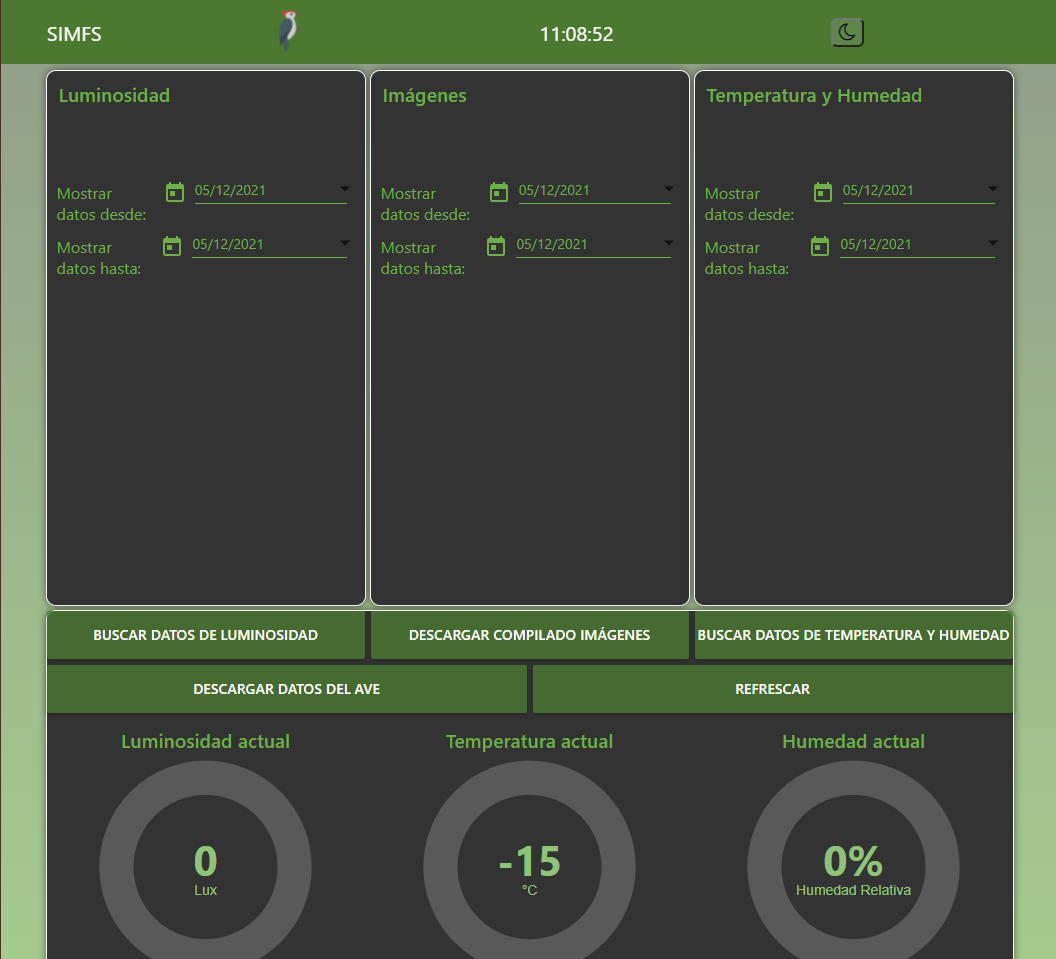
\includegraphics[width=\linewidth]{ImagenesIngenieria de Detalle/Node-Red-Dark}		
		\caption{Interfaz con usuario versión oscura.}
		\label{fig:front_end_dark}
	\end{subfigure}
	%\hfill	
	\begin{subfigure}[b]{0.49\textwidth}
		\centering
		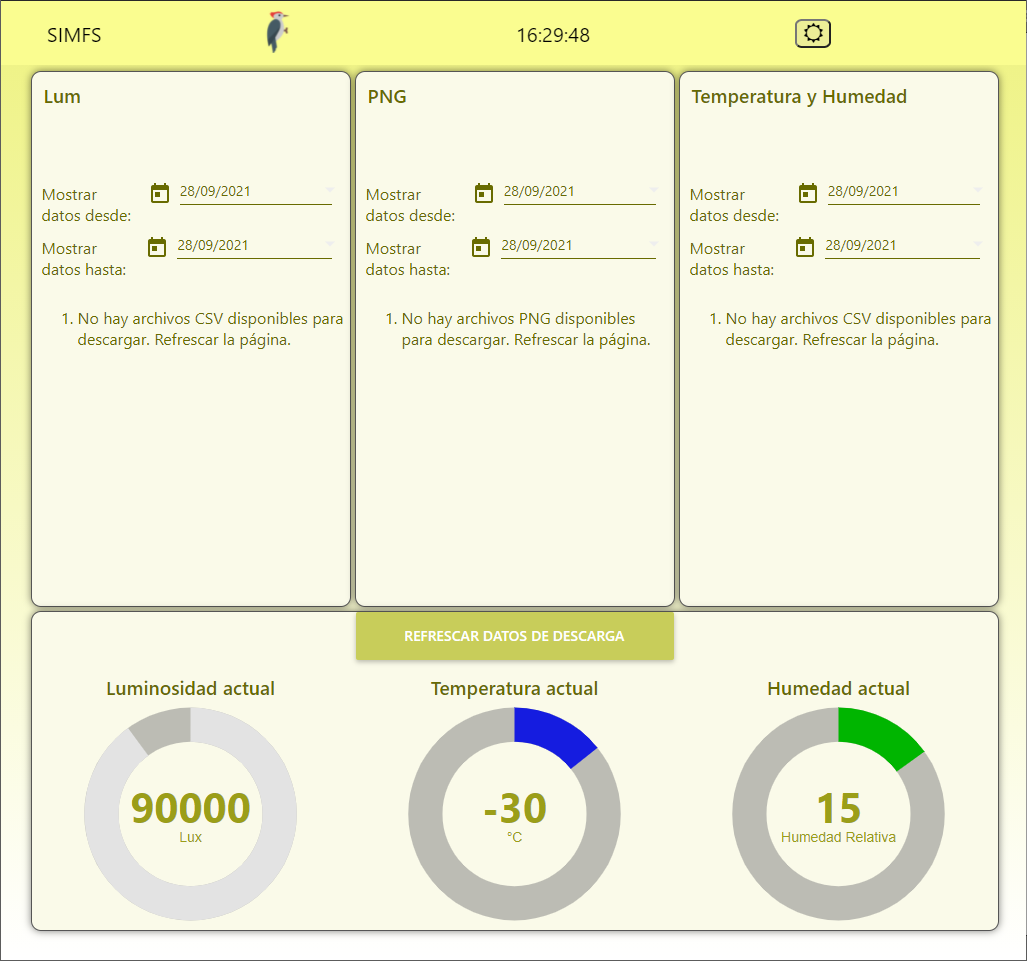
\includegraphics[width=\linewidth]{ImagenesIngenieria de Detalle/Node-Red-Light}		
		\caption{Interfaz con usuario versión clara.}
		\label{fig:front_end_light}
	\end{subfigure}	
	\caption{Página del servidor a la cual accede el usuario.}
	\label{fig:node_red}
\end{figure}

Finalmente, cabe destacar que el sistema de edición de la GUI puede ser accedido a través de un navegador de la misma manera que la interfaz del usuario. Para evitar que el usuario (o alguna persona no deseada) acceda a esta sección, se emplea un link privado, el cual es confidencial y no será brindado al usuario. También se vale del mismo sistema de autenticación que emplea la interfaz gráfica, creando un usuario único de administrador.

\begin{figure}[H]
	\centering
	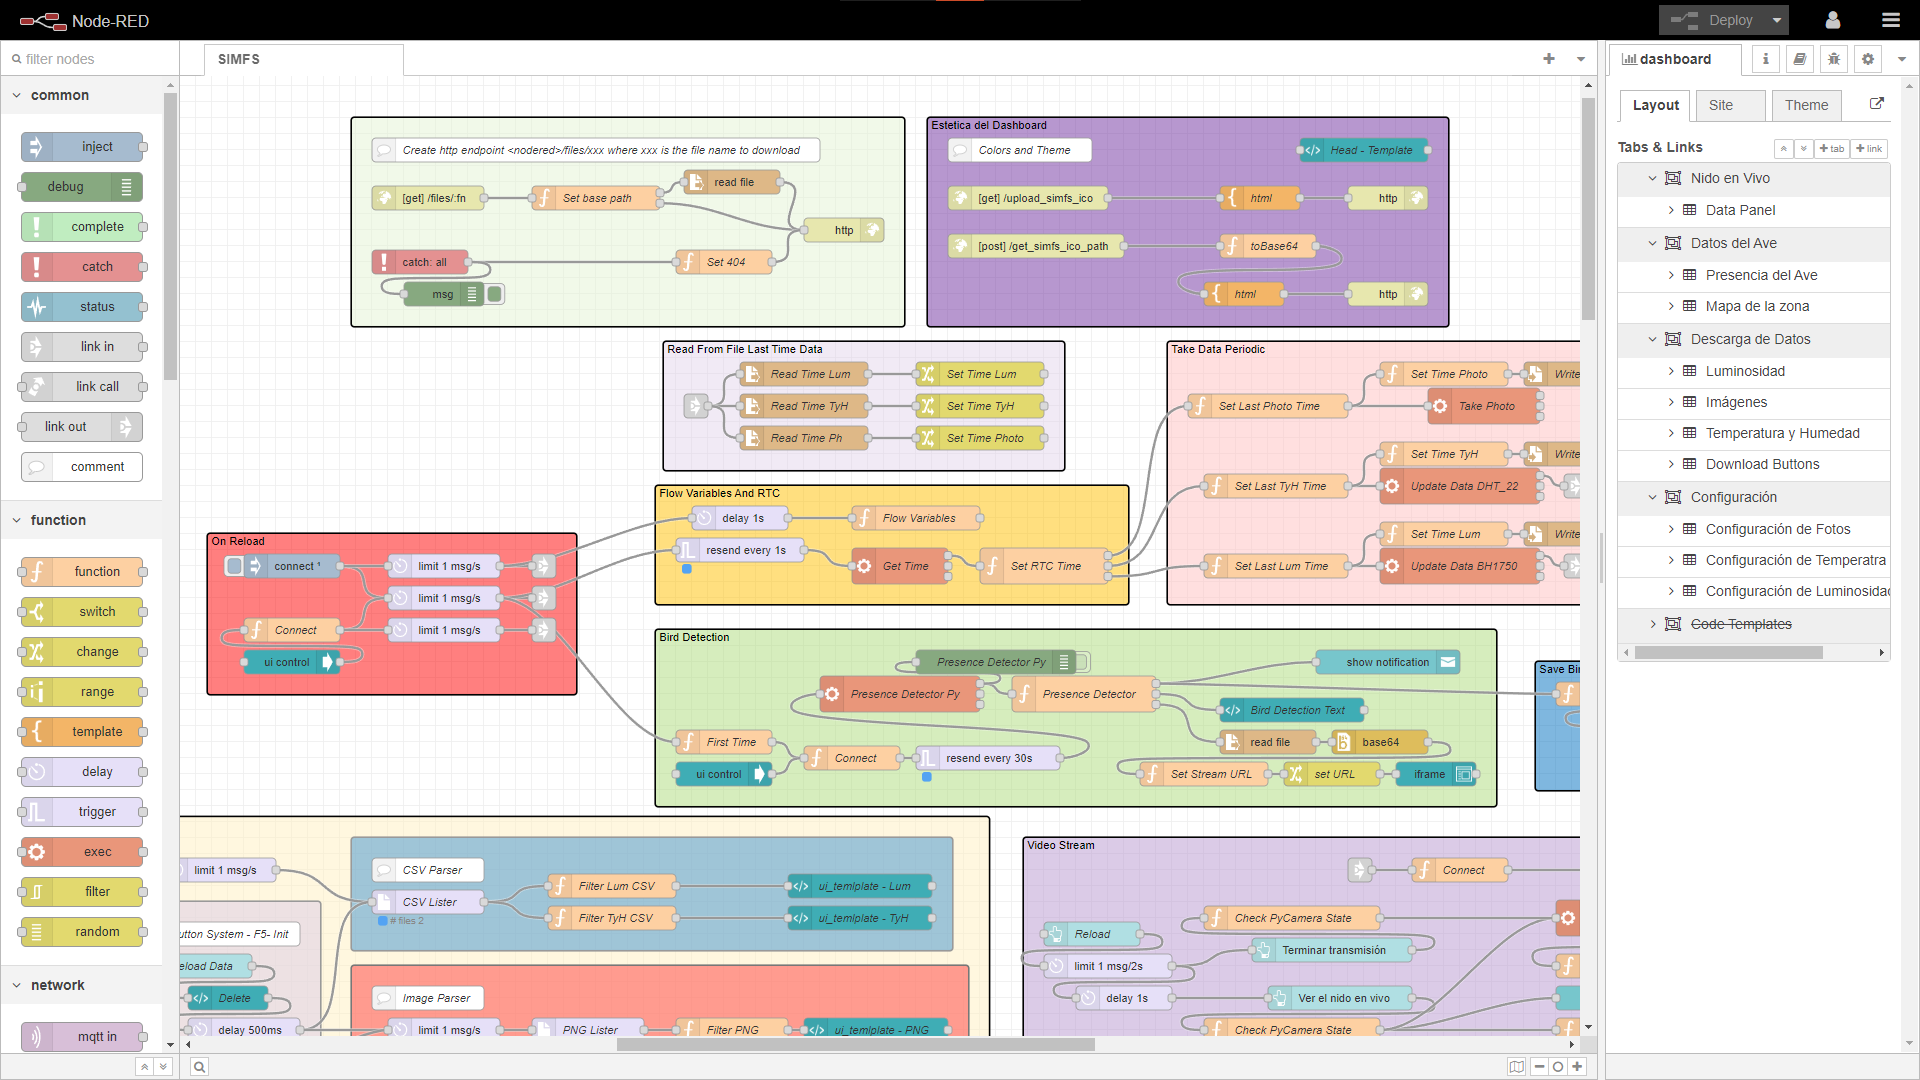
\includegraphics[width=0.9\linewidth]{ImagenesIngenieria de Detalle/Node-Red-Flow}
	\label{fig:node_red_flow}
	\caption{Flujo de nodos del servidor.}
\end{figure}